\section{启动停住时，从最后一行日志开始查}

“启动到内核”不是一根跳转箭头。控制权在 ROM、Stage 1、ELF loader 和 Kernel
之间交接；CPU 同时从实模式推进到保护模式和长模式；代码、页表、BootInfo、
staging 区和栈又必须占用互不冲突的物理内存。三条链有一条不成立，下一条
指令就可能不存在。

\begin{sidewaysfigure}[p]
  \centering
  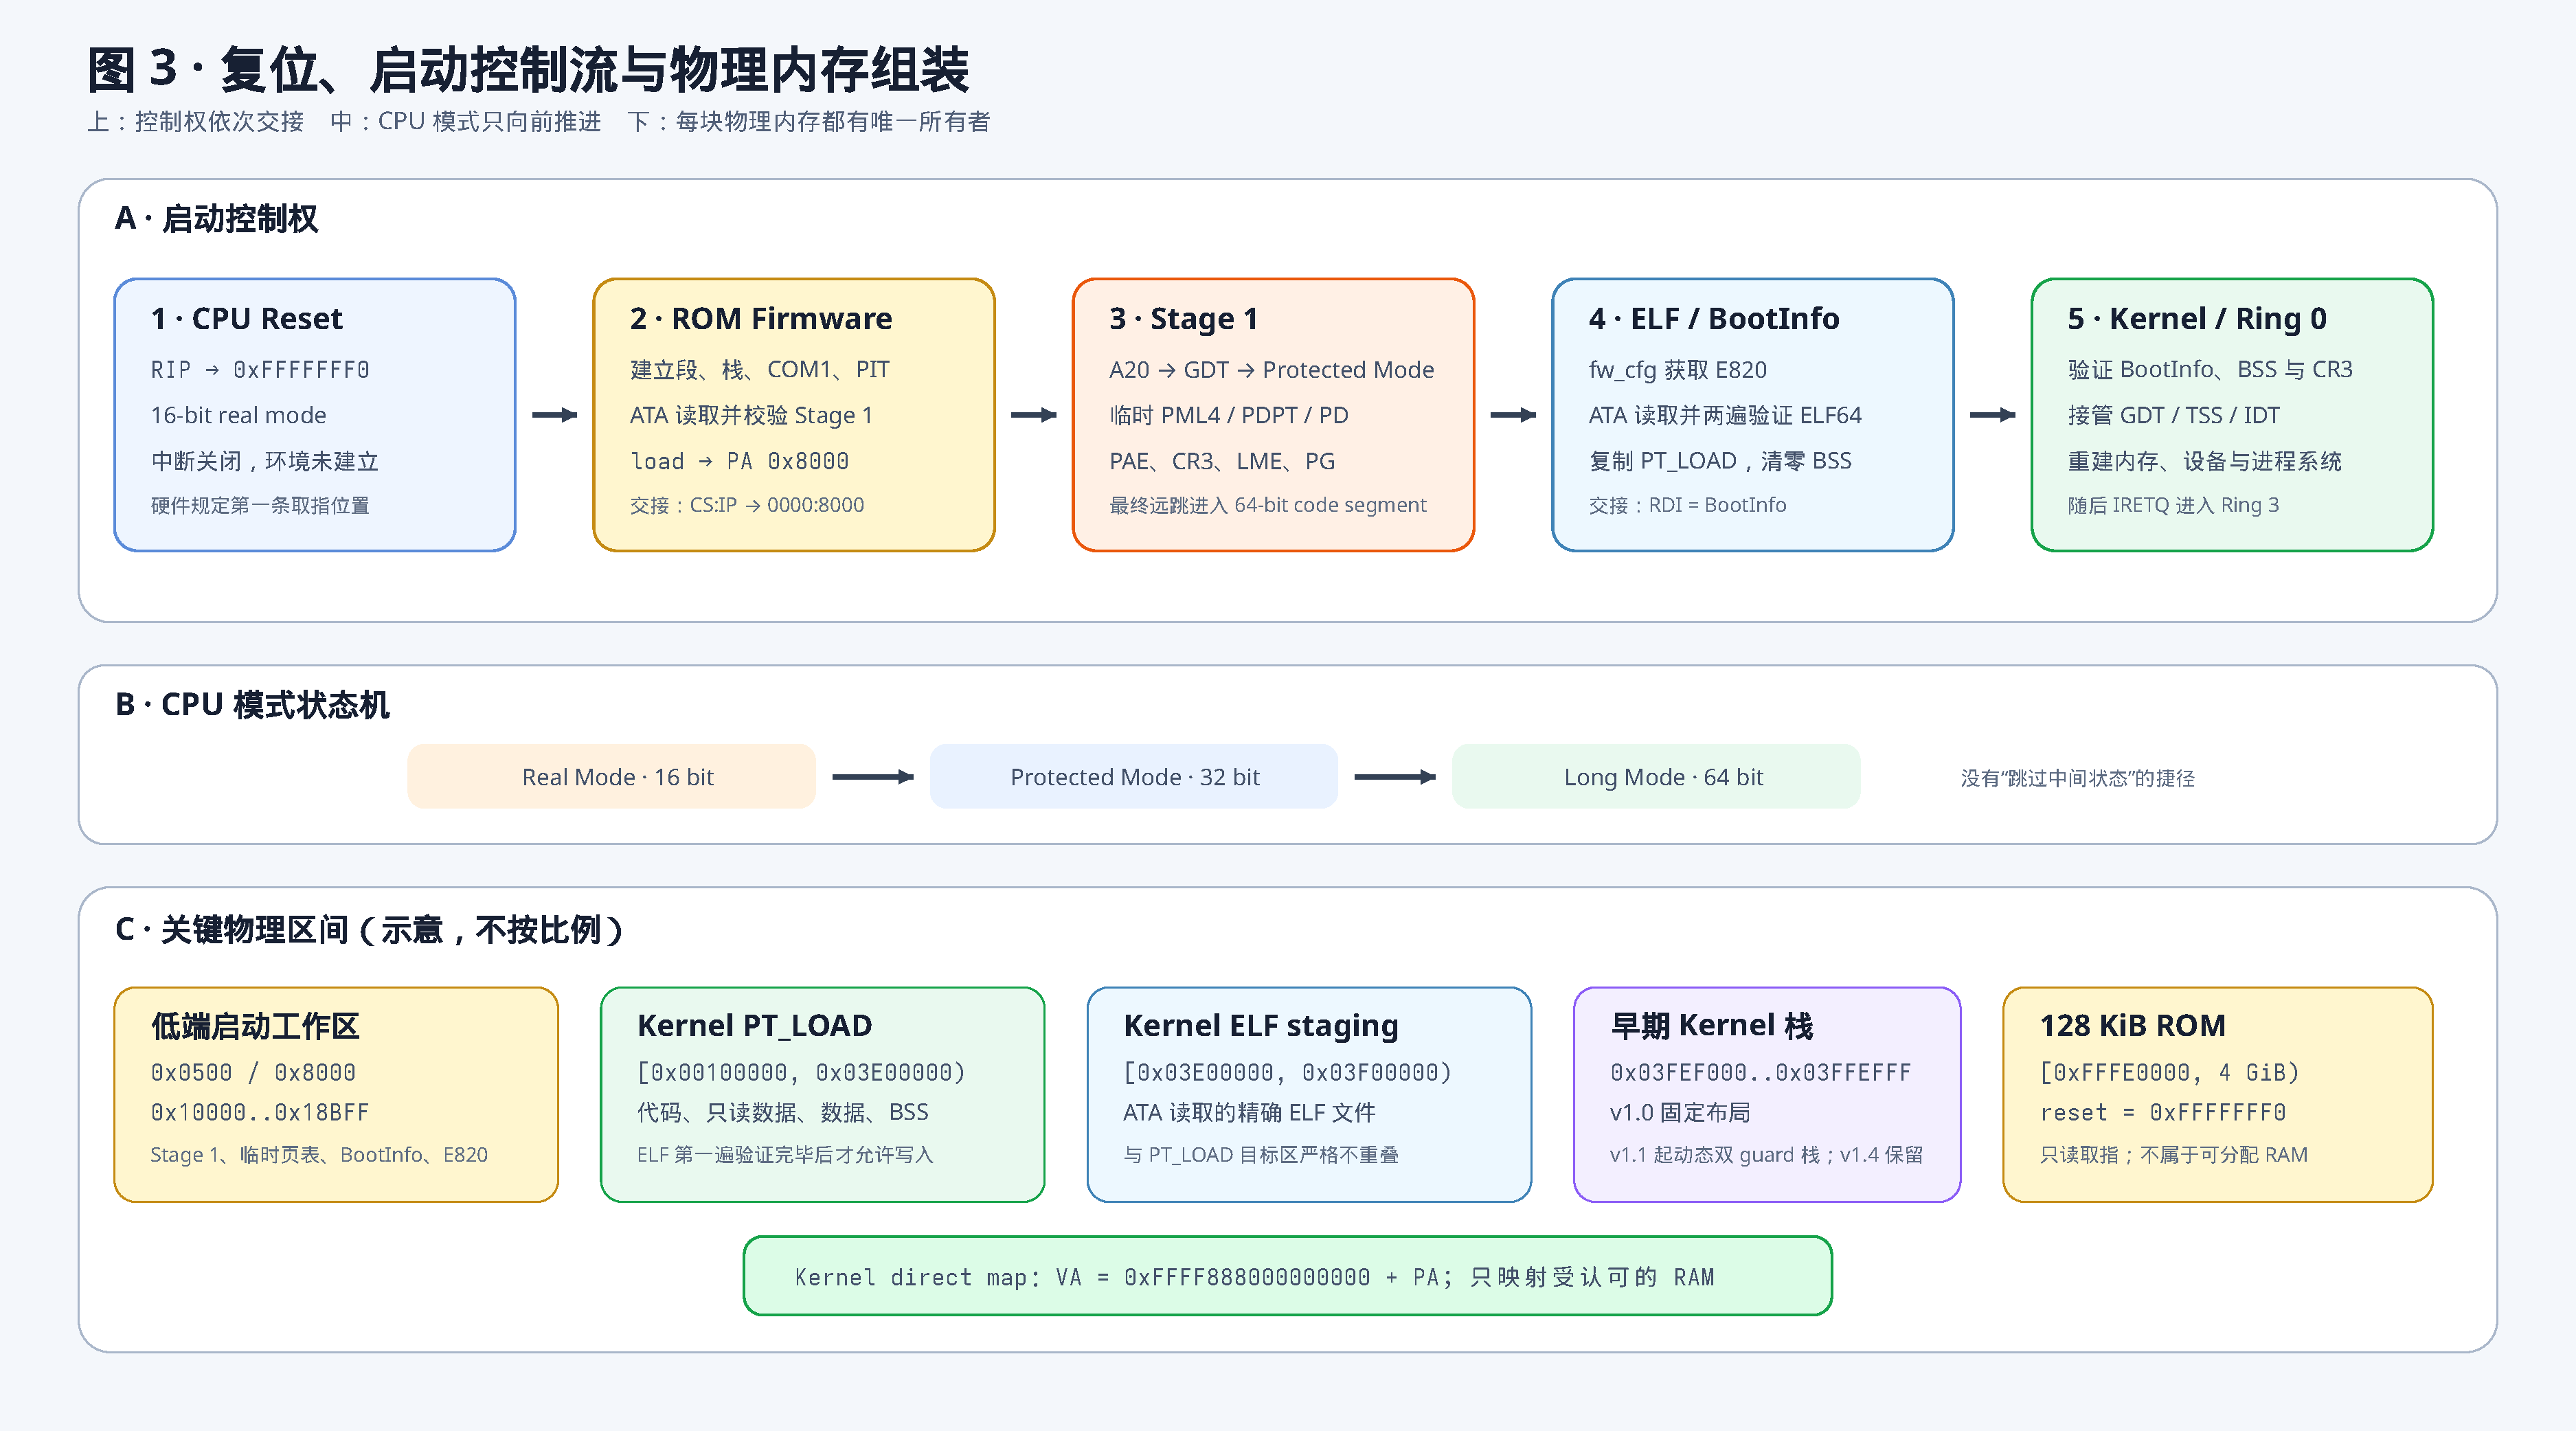
\includegraphics[width=0.96\textheight,height=0.82\textwidth,keepaspectratio]
    {figures/system_wiring/boot_and_memory_wiring.pdf}
  \caption{复位、启动控制流、CPU 模式状态和关键物理内存区间的统一矢量图。
  上层回答“谁把控制权交给谁”，中层回答“CPU 怎样解释下一条指令”，下层
  回答“字节具体放在哪里且归谁所有”。内存区间示意不按地址比例绘制。}
  \label{fig:boot-memory-wiring}
\end{sidewaysfigure}
\clearpage

\topic{1.1 CPU Reset 到 ROM Firmware}
复位时，CPU 把架构状态设置为规范值，并从复位向量附近取指。本项目的平台把
128 KiB ROM 映射到物理地址空间顶部，入口字节覆盖
\code{0xFFFFFFF0}。CPU 只承诺到这里取字节，不承诺字节合法、串口存在日志、
栈已建立或 RAM 内容为零。

ROM 入口首先关闭可屏蔽中断、清方向标志、重建段和栈，再配置 COM1。这样后续
每个危险步骤才有最小观测通道。若第一条串口标记都没有，调查范围应停在镜像
布局、复位向量、指令编码和最早 UART 初始化，而不是跳到内核 C++。

\topic{1.2 ROM Firmware 到 Stage 1}
固件经 ATA PIO 读取 Stage 1 描述符，验证尺寸和校验，再把字节搬到物理
\code{0x8000}。此时“磁盘里有 Stage 1”与“RAM 中已有可执行 Stage 1”是
两个不同事实；只有完整读取、验证和地址范围检查通过以后，固件才执行远控制
转移把 \code{CS:IP} 交给 \code{0000:8000}。

Stage 1 不是第二份固件硬件。它是已经位于 RAM 的软件阶段，获得了固件建立的
最小环境，也接过继续初始化处理器的责任。交接点必须冻结输入状态：当前模式、
段、栈、磁盘选择、数据位置和失败协议都不能靠双方各自猜测。

\topic{1.3 Stage 1 从实模式进入 64 位}
Stage 1 依次验证 A20、建立 GDT、设置保护模式、构造临时 PML4/PDPT/PD，
启用 PAE、写 CR3、设置 EFER.LME、开启分页，最后远跳转到 64 位代码段。
这条链中的箭头是依赖，不是建议顺序。比如 CR3 指向的页表若尚未写好，开启
分页后下一次取指就会使用垃圾翻译。

\topic{1.4 ELF/BootInfo 到 C++ Kernel}
进入 64 位不等于内核已经装入。Stage 1 从 \code{fw\_cfg} 获取并验证 E820
平台内存图，再从 ATA 读取 Kernel 容器与 ELF64。loader 第一遍检查全部
\code{PT\_LOAD} 的文件范围、目标范围、权限、对齐和互不重叠，只有整份输入
可接受时才开始第二遍复制，并把
\(\mathrm{p\_memsz}-\mathrm{p\_filesz}\) 对应的 BSS 清零。

\term{BootInfo}{启动交接结构}把版本、大小、内存图、磁盘和镜像等状态集中成
可验证 ABI。Stage 1 把其地址放入约定参数寄存器后调用 Kernel 入口。Kernel
第一步仍要重新验证版本、尺寸、范围和不变量，不能因为数据来自自家 loader
就放弃边界检查。

\topic{1.5 Kernel 接管以后}
Kernel 接管 GDT/TSS/IDT，验证页表和内存图，建立正式物理页分配、direct map、
堆、设备与进程系统。以后通过 \code{IRETQ} 进入 Ring 3，是另一次受控交接；
用户态不能继承 Ring 0 任意访问权限。图中最后一个框写“重建”，强调内核不会
永久依赖 Stage 1 的临时数据结构。

\topic{二、中层模式状态机为什么只允许向前提交}\par
\begin{osgridlongtable}{L{0.17\linewidth}L{0.24\linewidth}L{0.29\linewidth}L{0.20\linewidth}}
状态 & 主要地址/操作数能力 & 进入前必须准备 & 成功证据 \\ \hline
16 位实模式 & 段:偏移、兼容复位语义 & 已知段、栈、A20 与可观察串口 & 可执行受控 16 位路径 \\ \hline
32 位保护模式 & 描述符、32 位寄存器与控制状态 & GDT、合法代码段、CR0.PE & 远跳转后按 32 位入口取指 \\ \hline
64 位长模式 & 64 位寄存器、四级页表和 64 位代码段 & PAE 页表、CR3、LME、PG 与有效映射 & 64 位入口标记及规范寄存器状态 \\ \hline
\end{osgridlongtable}

“只向前”是本实现的设计约束：每一步先验证输入，提交一个最小状态改变，输出
标记，再准备下一步。x86 架构存在更多兼容和返回路径，但启动器不需要为了展示
所有可能性而增加回退状态；故障时停止并保留最后证据，比在半初始化环境里猜测
恢复更可靠。

\topic{模式不是源码文件的属性}%
NASM 的 \code{bits 16/32/64} 告诉汇编器如何编码，不能直接改变 CPU。CPU
是否按 64 位解释字节，取决于控制寄存器、EFER、分页状态和当前代码段属性。
反过来，在 CPU 已进入 64 位代码段后执行按 16 位意图编码的字节，可能被译码
为完全不同的指令并触发异常。

\topic{三、下层每块物理内存为什么必须只有一个当前所有者}
图中的物理区间不按大小比例绘制；它们表达的是用途和不可重叠关系。

\begin{osgridlongtable}{L{0.20\linewidth}L{0.23\linewidth}L{0.27\linewidth}L{0.20\linewidth}}
区域 & 典型内容 & 当前阶段所有者 & 不能发生的事情 \\ \hline
低端启动工作区 & Stage 1、临时页表、BootInfo、E820 staging & Firmware/Stage 1，交接后由 Kernel 保留或回收 & 互相覆盖或当普通空闲页分配 \\ \hline
Kernel \code{PT\_LOAD} & 代码、只读数据、数据与 BSS & Kernel 镜像 & loader 验证完成前部分写入 \\ \hline
Kernel ELF staging & 从磁盘读入的精确 ELF 文件字节 & Stage 1 loader & 与最终装载段重叠导致源被覆盖 \\ \hline
早期 Kernel 栈 & 进入内核时的临时/历史基线栈 & 当前执行流 & 在仍使用时撤映射或回收 \\ \hline
高地址 ROM & 固件代码、常量与复位入口 & 平台/ROM 镜像 & 当作可写 RAM 或可分配 frame \\ \hline
\end{osgridlongtable}

\term{所有者}{owner}说明当前谁有权解释、修改和最终释放一段存储，并不限制
知道地址的函数数量。staging 区在 ELF 复制完成前属于 loader；装载目标
成功提交后属于 Kernel 镜像；可用 E820 RAM 经保留区扣除并交给页分配器后，
才成为可分配 frame。所有权转换必须发生在明确提交点。

\topic{四、direct map 解决的是可访问性，不是所有权}
高半区 direct map 建立
\[
\mathrm{VA}=\mathrm{OS\_DIRECT\_MAP\_BASE}+\mathrm{PA}
\]
一类映射，使 Kernel 能用稳定虚拟地址访问经平台认可的物理 RAM。它没有把
reserved frame 变成 free，也不会让 MMIO、ROM 或 E820 hole 自动成为普通
缓存内存。页表回答“虚拟地址怎样到物理地址及允许什么访问”，页分配器回答
“这个物理 frame 当前归谁”，两者必须同时正确。

\topic{五、控制流、数据流和地址翻译怎样在同一步交汇}
以 loader 复制一个 \code{PT\_LOAD} 段为例：

\begin{enumerate}[leftmargin=2.2em]
  \item \textbf{控制流}：RIP 位于 Stage 1 的复制循环；
  \item \textbf{输入数据流}：ATA 已把 ELF 文件字节放在 staging 区；
  \item \textbf{地址规则}：程序头给出 file offset、目标地址和大小；
  \item \textbf{所有权}：staging 仍归 loader，目标区尚未提交给 Kernel；
  \item \textbf{写入动作}：CPU 从源 RAM 读取并写目标 RAM；
  \item \textbf{提交}：所有段复制和 BSS 清零成功，BootInfo 完整，才跳 Kernel。
\end{enumerate}

只画“ELF \(\rightarrow\) Kernel”会丢失 staging、地址验证和失败原子性；
只画内存布局又会丢失谁在何时执行复制。统一图的价值正是让三类问题相互约束。

\topic{六、最后标记怎样把三重故障缩小成一个区间}\par
\begin{osgridlongtable}{L{0.24\linewidth}L{0.31\linewidth}L{0.35\linewidth}}
最后成功边界 & 下一组重点检查 & 不应先做什么 \\ \hline
没有 ROM 首标记 & 复位向量、ROM 大小、入口机器码、最早 UART & 调试文件系统 \\ \hline
ROM 有、Stage 1 无 & ATA 描述符、LBA、校验、装载地址、远跳转 & 修改 Kernel C++ \\ \hline
保护模式有、长模式无 & GDT、PAE 页表、CR3、LME、PG、下一 RIP 映射 & 猜测 USB 驱动 \\ \hline
长模式有、Kernel 无 & ELF 容器、程序头、BSS、BootInfo、ABI 栈对齐 & 把问题都叫“三重故障” \\ \hline
Kernel 入口有、后续无 & 内核 GDT/TSS/IDT、内存图与正式页表接管 & 回头重写复位代码 \\ \hline
\end{osgridlongtable}

若错误让 CPU 无法交付异常，最终可能三重故障复位。串口标记不会告诉我们精确
错误位，却能证明此前所有边界已经通过，从而把调查限制在最后标记与下一标记
之间。书中测试还结合静态镜像审计、反汇编、故障注入和 QEMU 退出状态，使
“看起来启动了”变成可重复、可定位的证据。
